
\subsection{Impacto de remoción.}

\par En esta sección estudiamos el impacto de remover proteínas que son centrales bajo diferentes criterios y lo comparamos con el impacto de remover las proteínas catalogadas como esenciales. Según \cite{jeong2000}, un nodo con alto grado en la red de interacciones tiene más probabilidad de ser esencial que la esperada por azar, debido a que actúa de intermediario entre nodos de menor grado. Sin embargo, cabe la posibilidad de que no sea el número de vecinos inmediatos lo que determina la importancia de una proteína, sino algún otra propiedad topológica más global.
\par En las figura \ref{fig:remocion} estudiamos cómo se modifica el tamaño relativo (al tamaño de la componente de la red original) de la componente más grande al remover los nodos catalogados como centrales según diferentes criterios, para las cuatro redes estudiadas. Comparamos estos resultados con el caso de remover las proteínas esenciales, y con remover nodos al azar sin más criterio. Los criterios utilizados fueron: grado del nodo, centralidad de betweenness, centralidad de Bonacich, y subgraph centrality. 
\par De la figura \ref{fig:remocion} concluímos que el impacto de remoción de nodos centrales es mayor que la remoción de los nodos esenciales, que en algunos casos es equivalente a remover nodos al azar. Esto daría la noción que la esencialidad de una proteína no está ligada exclusivamente a su rol en la red de interacciones.
\par Cabe destacar que el proceso de remoción consistió en calcular la centralidad de cada nodo en la red original, y removerlos de mayor a menor sin volver a realizar el cálculo. Esto implica que removimos los nodos que son centrales en la red original. Si se decide remover el nodo con mayor centralidad luego de realizar una remoción, el impacto de la misma es mayor que el criterio que utilizamos, sin embargo le daríamos el rol de central a un nodo que quizás no lo cumple en la red original. A modo de criterio alternativo, incluímos un gráfico análogo a \ref{fig:remocion} en la figura \ref{fig:remocion_alternativo}, donde se puede observar que el impacto de remoción es mayor.
 
\begin{figure}
\centering
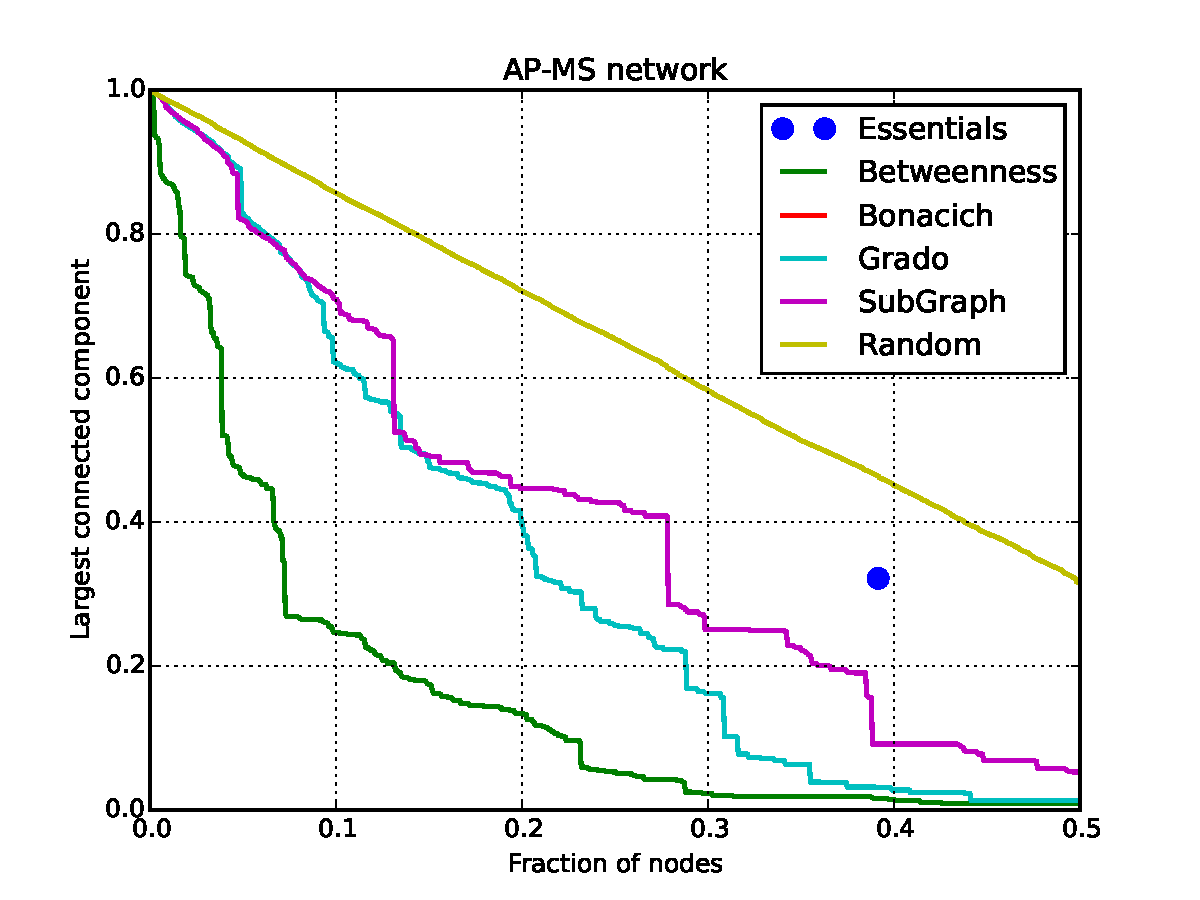
\includegraphics[scale = 0.3]{figuras/AP-MS_b-eps-converted-to} 
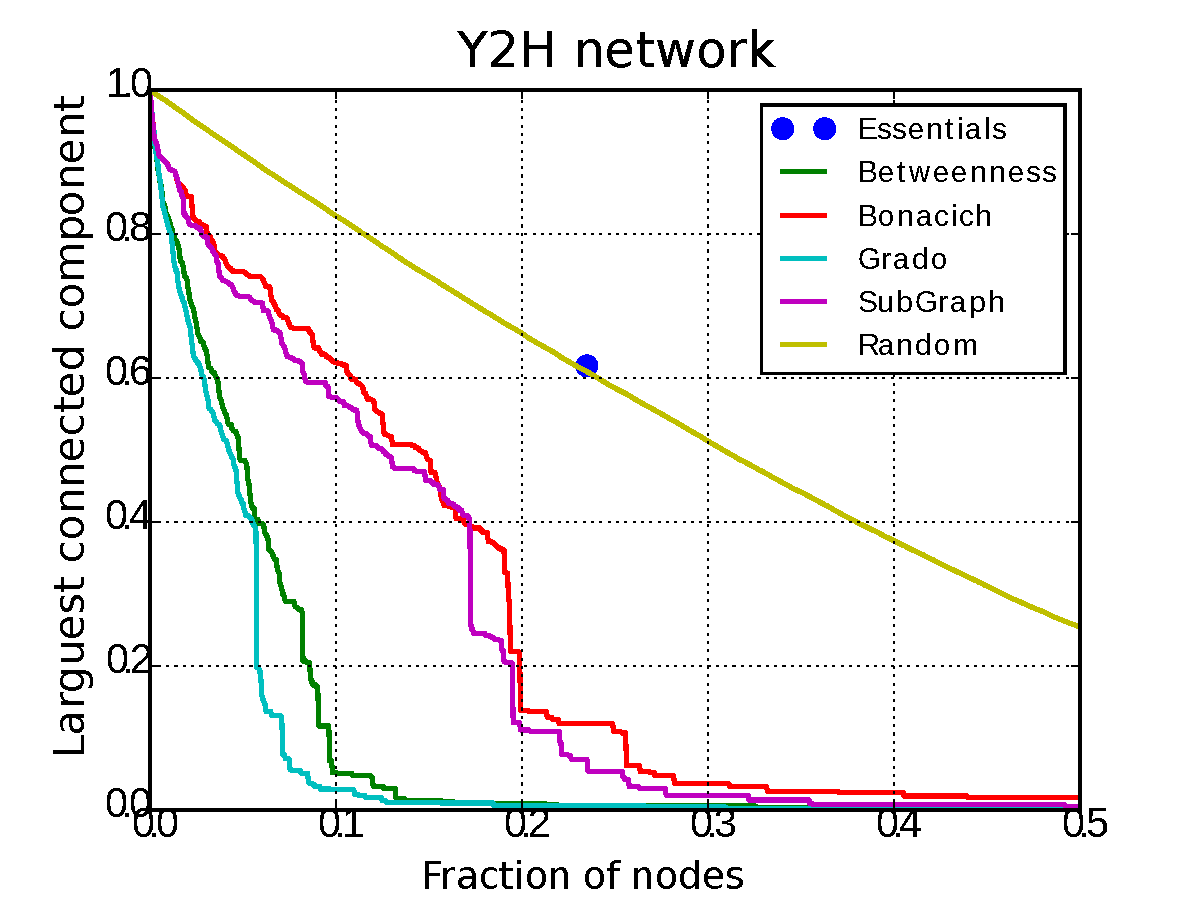
\includegraphics[scale = 0.3]{figuras/Y2H_b-eps-converted-to} \\
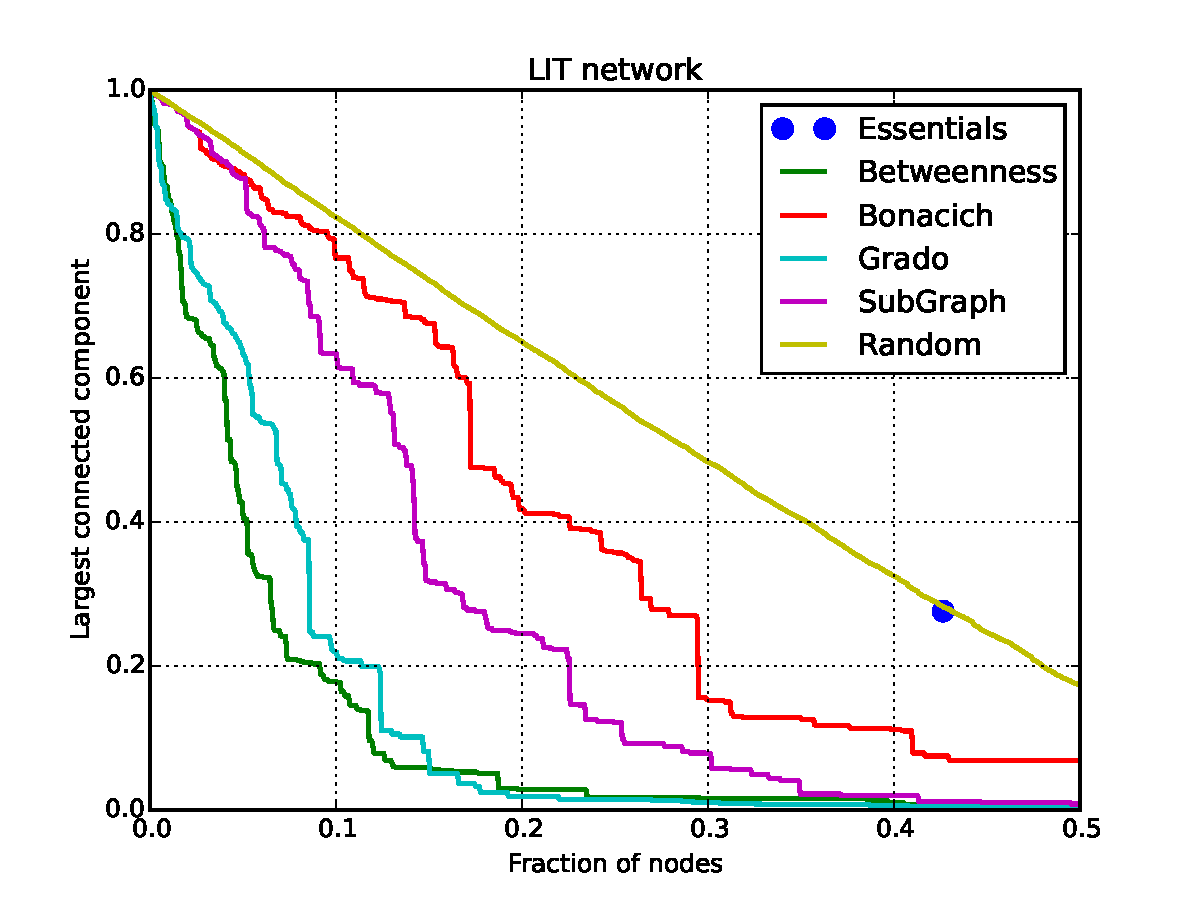
\includegraphics[scale = 0.3]{figuras/LIT_b-eps-converted-to} 
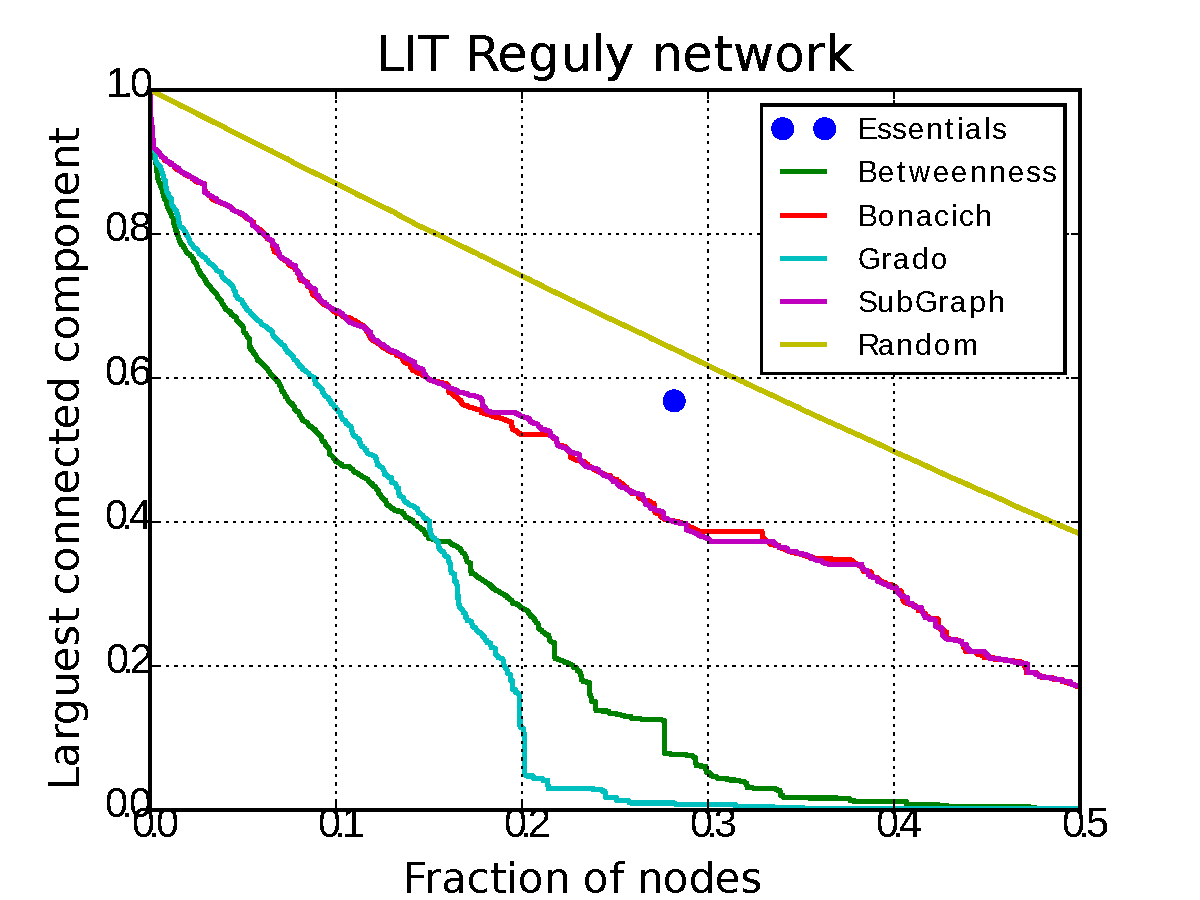
\includegraphics[scale = 0.3]{figuras/LIT_Reguly_b-eps-converted-to} 
\caption{Tamaño relativo de la componente conectada más grande a medida que se remueven los nodos ordenados con diferentes criterios de centralidad. Se incluye el impacto de remover las proteínas esenciales y remover nodos al azar. En todos los casos se puede observar que el impacto de remoción (caída del tamaño del fragmento conectado) es mucho más alto al utilizar un criterio de centralidad en comparación con la remoción de las esenciales, que en algunos casos, prácticamente coincide con la remoción al azar.}
\label{fig:remocion}
\end{figure}

\begin{figure}
\centering
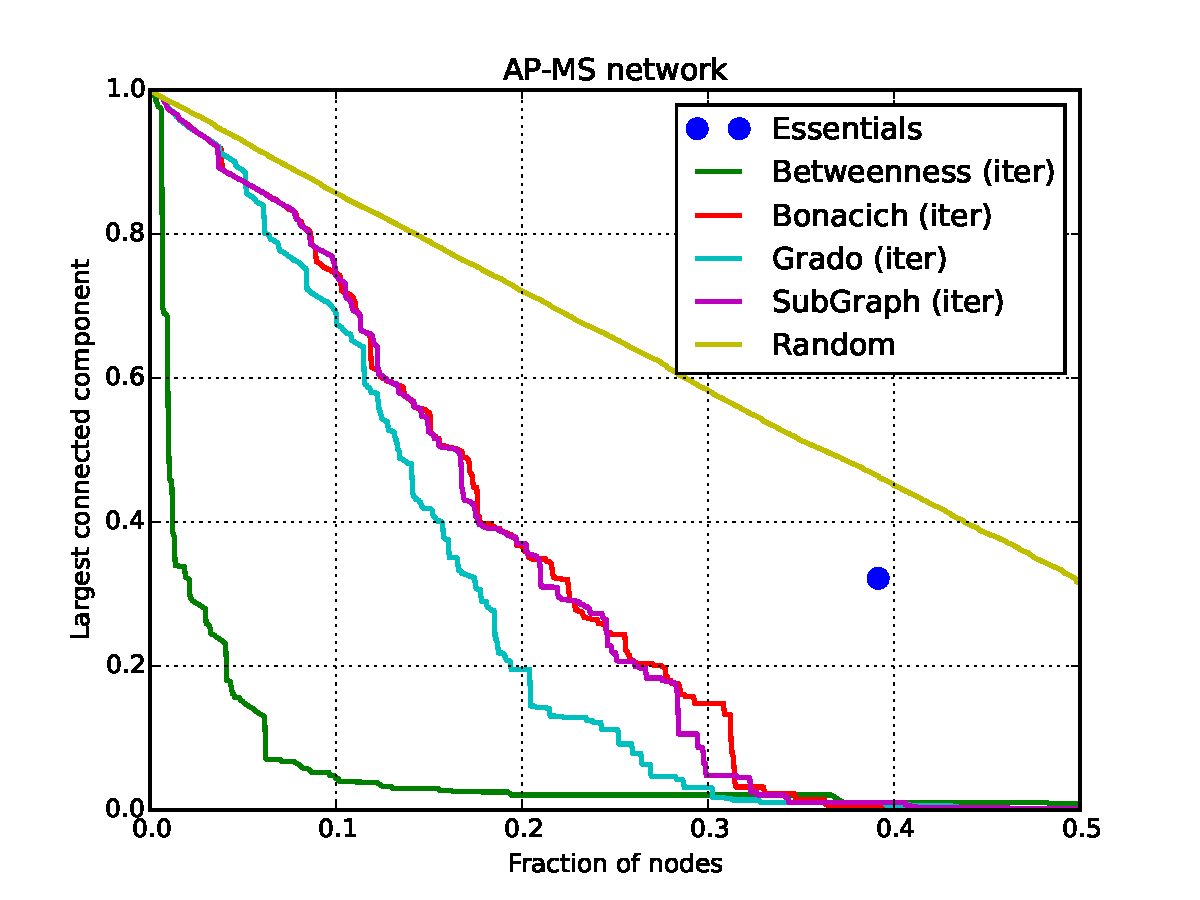
\includegraphics[scale = 0.3]{figuras/AP-MS-eps-converted-to} 
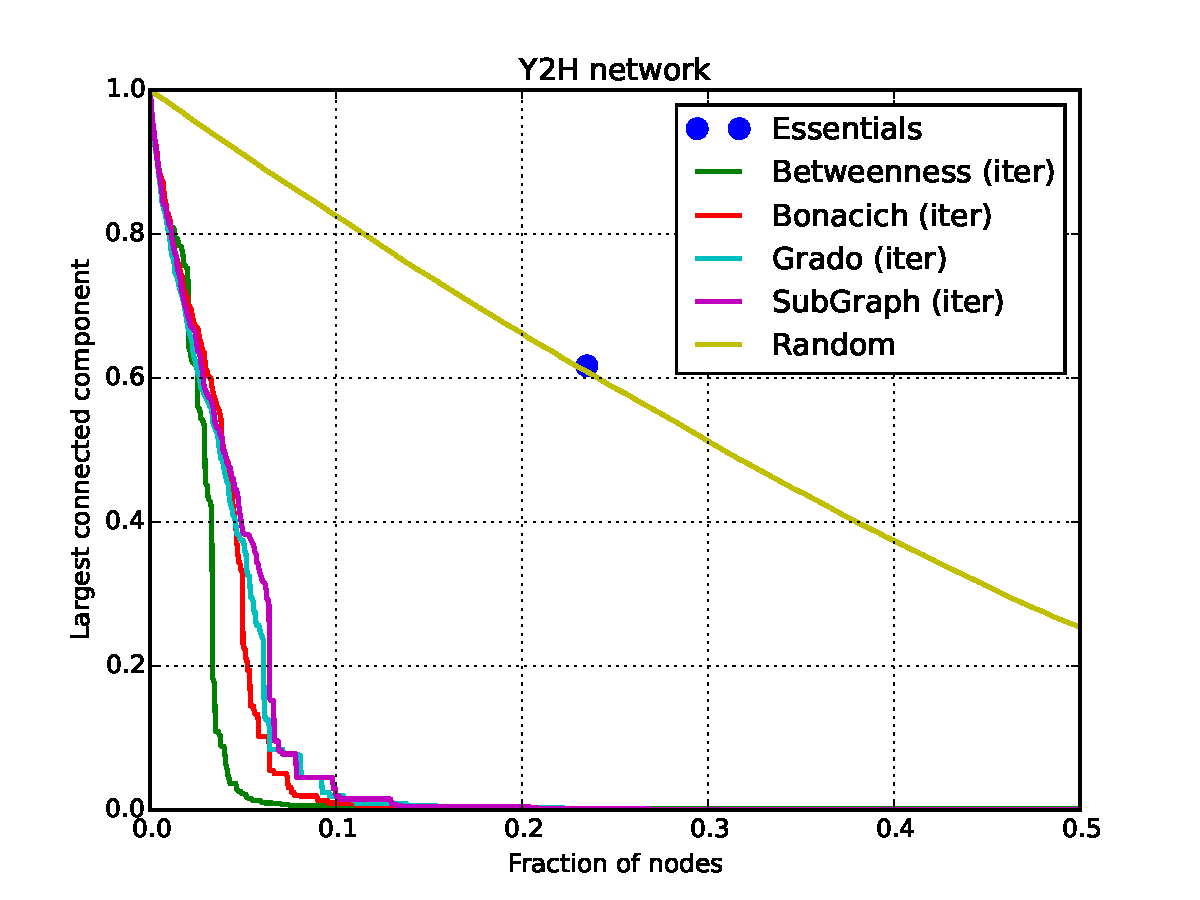
\includegraphics[scale = 0.3]{figuras/Y2H-eps-converted-to} \\
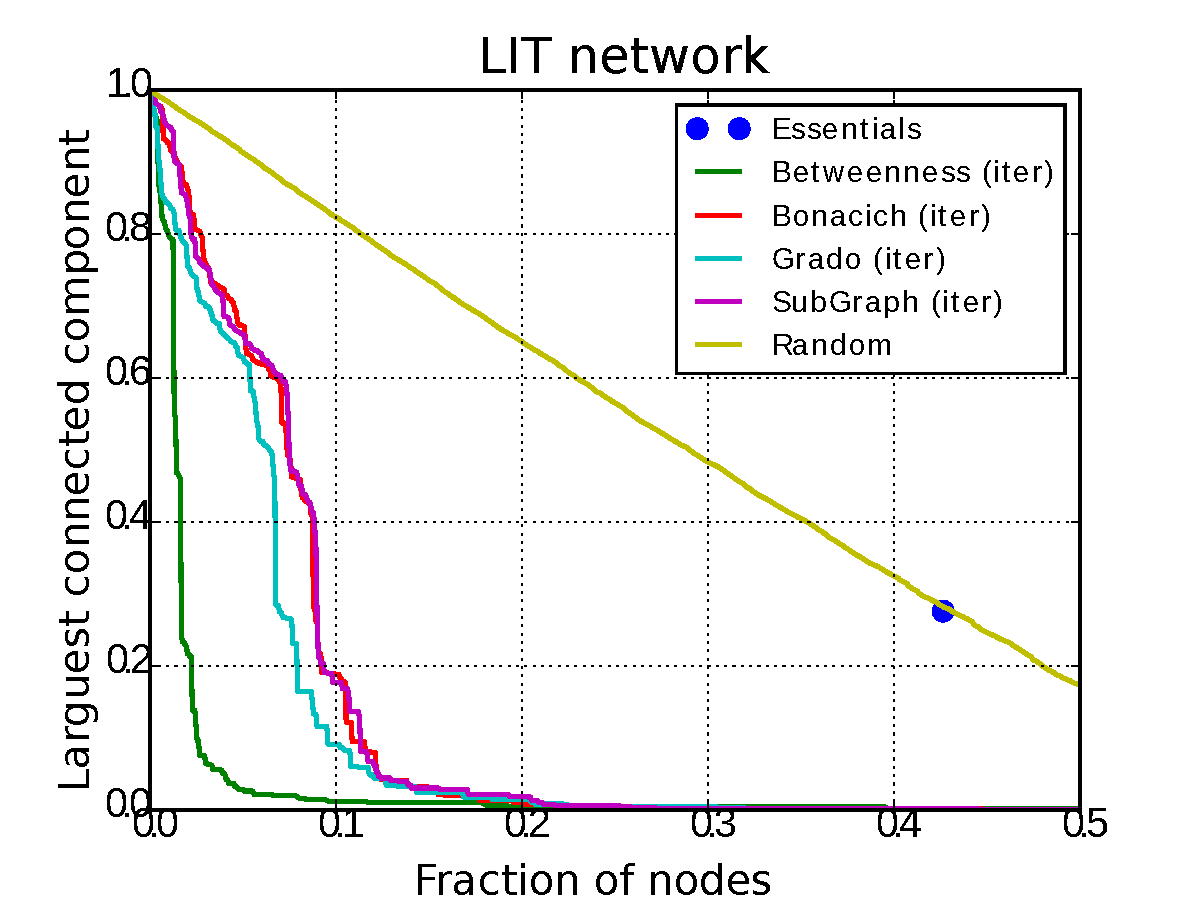
\includegraphics[scale = 0.3]{figuras/LIT-eps-converted-to} 
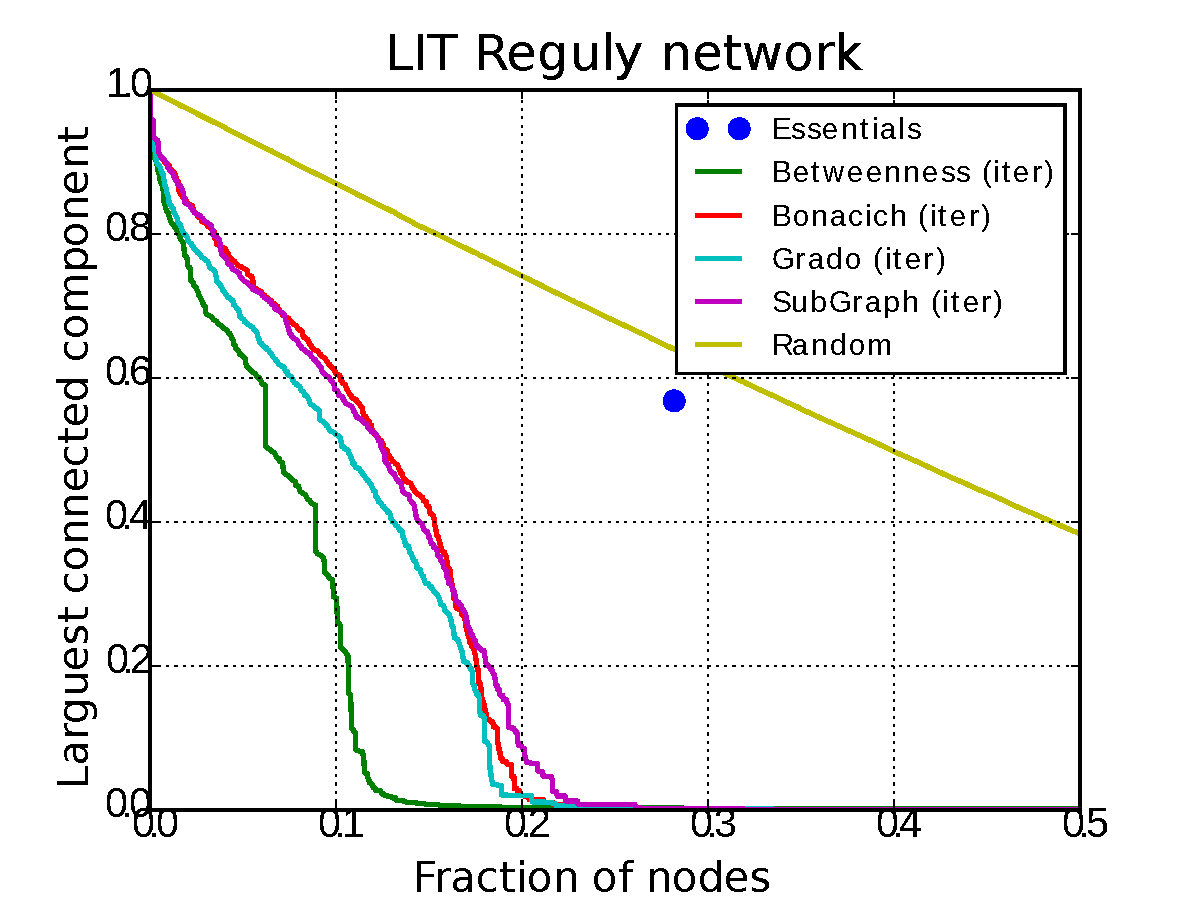
\includegraphics[scale = 0.3]{figuras/LIT_Reguly-eps-converted-to} 
\caption{Tamaño relativo de la componente conectada más grande a medida que se remueven los nodos ordenados con diferentes criterios de centralidad, en forma iterativa, es decir, se remueve el nodo más central en la configuración actual de la red. Se puede observar que el impacto de remoción es mayor que el de la figure \ref{fig:remocion}.}
\label{fig:remocion_alternativo}
\end{figure}

\subsubsection{Remoción de nodos al azar.}

\par En las figuras \ref{fig:remocion} y \ref{fig:remocion_alternativo}, la remoción de nodos al azar no siguió ningún criterio particular. En esta sección estudiaremos el impacto de tomar nodos al azar no esenciales y cuya distribución de grado sea equivalente a la de los nodos esenciales presentes en la red. Tomaremos nuevamente el tamaño relativo de la componente más grande como impacto de remoción. Cabe recordar que un tamaño relativo menor implica un impacto de remoción mayor.
\par En la tabla \ref{table:remocion}, comparamos el impacto de remover los nodos esenciales con la remoción de nodos no esenciales, con distribución de grado equivalente. El criterio tomado consistió en, dado un nodo esencial, tomar uno no esencial con el grado más cercano posible.
\begin{table}
\centering
\begin{tabular}{c c c c}
\hline \hline
Red & Tr(Esenc.) & Tr(No Esenc.) & Nodos removidos \\
\hline
AP-MS & 0.32 & $0.38 \pm 0.02$ & 615 \\
LIT & 0.276 & $0.417 \pm 0.003$ & 636 \\
Y2H & 0.62 & $0.61 \pm 0.01$ & 459 \\
LIT-Reguly & 0.568 & $0.536 \pm 0.005$ & 903 \\
\hline\hline
\end{tabular}
\caption{Tamaño relativo de la componente conectada más grande al remover proteínas esenciales, y nodos no esenciales con distribución de grado equivalente.}
\label{table:remocion}
\end{table}
\par De la tabla podemos concluir que en las redes Y2H y LIT-Reguly, el impacto de remoción es prácticamente el mismo que remover nodos no esenciales con la misma distribución de grado, e incluso el impacto es levemente mayor para la segunda red. Sin embargo, para las redes restantes, y con mayor notoriedad en la red LIT, la remoción de las proteínas esenciales es más dañina que la remoción de nodos al azar. Si observamos la figura \ref{fig:remocion} para la red LIT, la remoción de nodos al azar sin ningún criterio es prácticamente igual a remover los esenciales. Cabe destacar que en la construcción de la figura \ref{fig:remocion} al tomar nodos al azar se incluyeron a las proteínas esenciales, lo cual, la tabla podría indicar que en esta red algunas proteínas esenciales cumplen algún rol de centralidad.
\par Del estudio de impacto de remoción concluímos entonces, que ciertas proteínas no son esenciales exclusivamente por su rol topológico en la red, debido a que remover aquellos nodos que cumplen cierto grado de centralidad es siempre más dañino para la red que la remoción de las catalogadas como esenciales. Incluso en algunas de las redes, el impacto de remover nodos al azar es equivalente a la remoción de las esenciales.


